%%%%%%%%%%%%%%%%%%%%%%%%%%%%%%%%%%%%%%%%%
% Journal Article
% LaTeX Template
% Version 1.4 (15/5/16)
%
% This template has been downloaded from:
% http://www.LaTeXTemplates.com
% Frits Wenneker, Vel
%
% License:
% CC BY-NC-SA 3.0 (http://creativecommons.org/licenses/by-nc-sa/3.0/)
%
%%%%%%%%%%%%%%%%%%%%%%%%%%%%%%%%%%%%%%%%%

\documentclass[twoside,twocolumn]{article}

\usepackage[sc]{mathpazo}
\usepackage[T1]{fontenc}
\linespread{1.05}
\usepackage{microtype}
\usepackage[english]{babel}
\usepackage[hmarginratio=1:1,top=32mm,columnsep=20pt]{geometry}
\usepackage[hang, small,labelfont=bf,up,textfont=it,up,tableposition=top]{caption}
\usepackage{booktabs}
\usepackage[version=4]{mhchem}
%\usepackage[backend=bibtex,style=verbose-trad2]{biblatex}

\usepackage{enumitem}
\newlist{abbrv}{itemize}{1}
\setlist[abbrv,1]{label=,labelwidth=1in,align=parleft,itemsep=0.1\baselineskip,leftmargin=!}

\usepackage{abstract}
\renewcommand{\abstractnamefont}{\normalfont\bfseries}
\renewcommand{\abstracttextfont}{\normalfont\small\itshape}

\usepackage{titlesec}
\renewcommand\thesection{\Roman{section}}
\renewcommand\thesubsection{\arabic{subsection}}
\titleformat{\section}[block]{\large\scshape\centering}{\thesection.}{1em}{}
\titleformat{\subsection}[block]{\large}{\thesubsection.}{1em}{}

\usepackage{fancyhdr}
\pagestyle{fancy}
\fancyhead{}
\fancyfoot{}
\fancyfoot[RO,LE]{\thepage}

\usepackage{titling}
\usepackage{hyperref}
\usepackage{graphicx}
\usepackage{cuted}


%----------------------------------------------------------------------------------------
%	TITLE SECTION
%----------------------------------------------------------------------------------------

\setlength{\droptitle}{-4\baselineskip}

\pretitle{\begin{center}\Huge\bfseries}
\posttitle{\end{center}}
\title{Dopamine modulation of Glutamate sinaptic plasticity}
\author{
\textsc{The laboratory of Machine Thinking} \\[1ex]
\normalsize ITIS
}
\date{03 July 2017}
\renewcommand{\maketitlehookd}

%----------------------------------------------------------------------------------------

\begin{document}


\maketitle

%----------------------------------------------------------------------------------------
%	ARTICLE CONTENTS
%----------------------------------------------------------------------------------------

\section{Symbols and Abbreviations}
\begin{strip}
\begin{abbrv}
\item[E]                   Enzyme
\item[A]                   Substrate
\item[P]                   Product
\item[ODE]                 Ordinary Differential Equation(s)
\item[D1]                  Dopamine receptors of type D1
\item[D2]                  Dopamine receptors of type D2
\end{abbrv}
\end{strip}

\section{Synaptic weight formulas}
\begin{strip}
According to \cite[p.~20]{gurney_new_2015} the change of synaptic weight $w$ can be calculated as:
\[ \frac{dw}{dt} = \mu(z^{+}_{D}[d(t),\Delta t] + z^{-}_{D}[d(t),\Delta t])\exp(-t/\tau_{g}) \]
where:
\[ z^{\pm}_{D}[d(t),\Delta t] = z^{\pm}_{D1}[d(t),\Delta t] + z^{\pm}_{D2}[d(t),\Delta t]\]
$z[d(t),\Delta t]$ for $D1$ and $D2$ can be described by the same function. Differences between receptors can be set by different values of functions' coefficients. This allows us to omit $Di$ subscript in the upcoming $z$ definition.
\[ z^{\pm}[d(t),\Delta t] = \alpha(d)z^{\pm}_{hi}(\Delta t) + (1 - \alpha(d))z^{\pm}_{lo}(\Delta t) \]
\[ z^{+}_{lo}(\Delta t) = k^{+}_{lo}s^{+}(\Delta t) , s^{+}(\Delta t) = \exp(-\Delta t/\tau) \]
\[ z^{-}_{lo}(\Delta t) = k^{-}_{lo}s^{-}(\Delta t) , s^{-}(\Delta t) = \exp(\Delta t/\tau) \]
\[ z^{+}_{hi}(\Delta t) = k^{+}_{hi}s^{+}(\Delta t) , s^{+}(\Delta t) = \exp(-\Delta t/\tau) \]
\[ z^{-}_{hi}(\Delta t) = k^{-}_{hi}s^{-}(\Delta t) , s^{-}(\Delta t) = \exp(\Delta t/\tau) \]
\[ \alpha = \frac{\alpha_{0}d^{p}}{d^{p} + \theta^{p}} \]

\begin{tabular}{|l|*{4}{c|}}
  \hline
   \ $t$ &$\Delta t$        &$\mu$&$\tau_{g}$&$\tau$ \\ \hline
   \ time&$t_{post}-t_{pre}$&0.65 &0.3       &0.02   \\ \hline
\end{tabular}
\begin{tabular}{|l|*{7}{c|}}
  \hline
   \   & $k^{+}_{lo}$ & $k^{-}_{lo}$ & $k^{+}_{hi}$ & $k^{-}_{hi}$ & $p$ & $\theta$ & $a_{0}$ \\ \hline
   \ D1 & -0.4        & -0.5         & 1.3          & 0            & 1.2 & 6.0      & 1.2     \\ \hline
   \ D2 & 0.3         & 0.3          & 0.35         & -0.85        & 1.4 & 1.8      & 1.0     \\ \hline
\end{tabular}
\end{strip}

\section{Kinetic pathways diagram}

%TODO Redraw diagram of pathways by TikZ http://www.texample.net/tikz/examples/tag/diagrams/

\begin{strip}
    \centering\noindent
    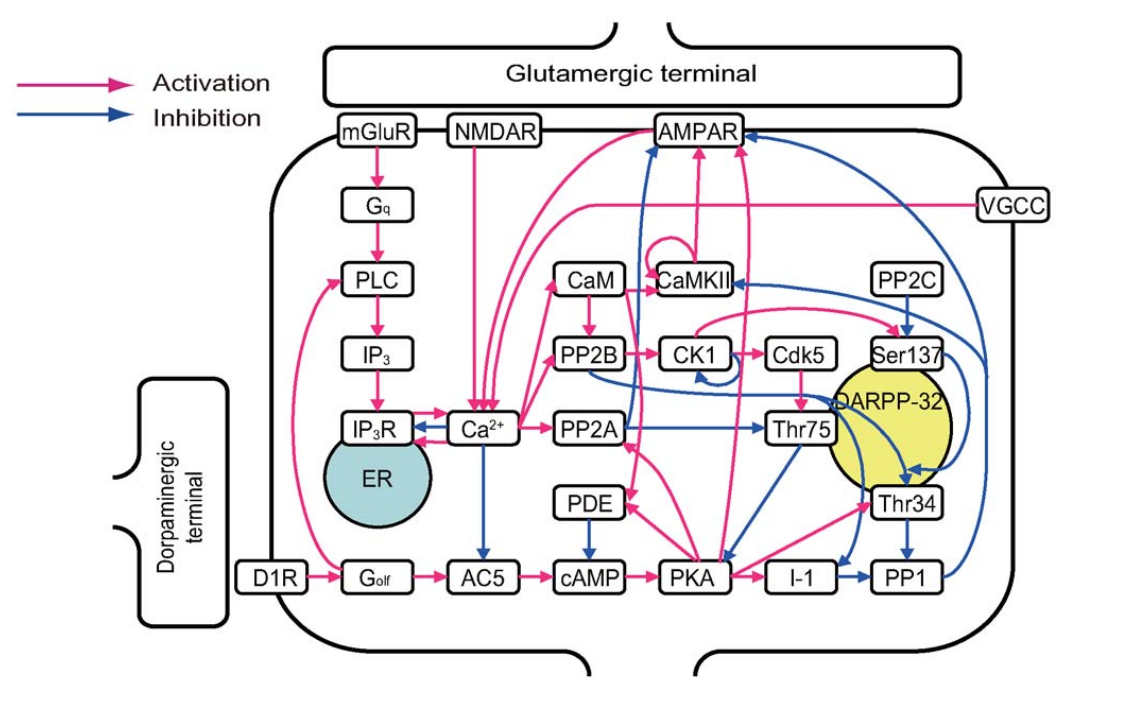
\includegraphics[width=\textwidth,natwidth=1132,natheight=701]{dopamine-kinetic-diagram.png}
    \captionof{figure}{Kinetic pathways taken from \cite{nakano_kinetic_2010}.}
\end{strip}

\section{Kinetic pathways}
\subsection{Glu to mGluR}
Binding of Glutamate to its Metabotropic receptors.
\\\ce{Glu + mGluR <=>[k1][k_{-1}] {Glu.mGluR}}
\\Kinetics Type: ~\ref{subsec:enzyme_binding}
\\Coefficients: $k_{1}$: ?, $k_{-1}$: ? 

\subsection{Glu.mGluR to \texorpdfstring{G\textsubscript{q}}{Gq}}
Release of $G_{q}$ from $Glu.mGluR$.
\\\ce{G_{\alpha\Beta\gamma} + Glu.mGluR <=>[k1][k_{-1}] {GGlu.mGluR} ->[k2] Glu.mGluR + G_{q\alpha}}
\\Kinetics Type: ~\ref{subsec:enzyme_irreversible} or ~\ref{subsec:enzyme_michaelis}
\\Coefficients: $k_{1}$: ?, $k_{-1}$: , $k_{2}$: ? 

\section{Enzyme kinetics}
\subsection{Binding reaction}
\label{subsec:enzyme_binding}
\ce{A + E <=>[k1][k_{-1}] {EA}}
\\\\This is an equation of binding substrate to enzyme \cite[p.~135]{sterratt_principles_2011}. Under the assumption of \textbf{well-mixed system}\cite[p.~135]{sterratt_principles_2011} the solution to this equation can be written as a group of ODE according to \textbf{the law of mass action}\cite[p.~10]{bisswanger_enzyme_2002}:
\[ \frac{d[A]}{dt} = -k_{1}[A][E] + k_{-1}[EA]\]
\[ \frac{d[EA]}{dt} = k_{1}[A][E] - k_{-1}[EA]\]
From $k_{1}$ and $k_{-1}$ we can define \textit{Association} constant $K_{a}$ and \textit{Dissociation} constant $K_{d}$.
\[ K_{a} = \frac{k_{1}}{k_{-1}} = \frac{[EA]}{[E][A]} \]
\[ K_{d} = \frac{k_{-1}}{k_{1}} = \frac{[E][A]}{[EA]} \]

\subsection{General reaction}
\label{subsec:enzyme_general}
\ce{A + E <=>[k1][k_{-1}] {EA} <=>[k2][k_{-2}] {EP} <=>[k3][k_{-3}] E + P}
\\\\This is an equation of general enzyme reaction. It's not used for modelling but you should understand that the correct representation of enzyme reaction is described in this way. 

\subsection{Reversible reaction}
\label{subsec:enzyme_reversible}
\ce{A + E <=>[k1][k_{-1}] {EA} <=>[k2][k_{-2}] E + P}
\\In this equation we omit the second step and assume that AE complex dissociates onto E and P directly. See Reversible Enzyme reactions \cite[p.~75]{bisswanger_enzyme_2002}. Under the assumption of \textbf{well-mixed system} the solution to this equation can be written as a group of ODE according to \textbf{the law of mass action}:
\[ \frac{d[A]}{dt} = -k_{1}[A][E] + k_{-1}[EA]\]
\[ \frac{d[E]}{dt} = -k_{1}[A][E] - k_{-2}[E][P] + (k_{-1} + k_{2})[EA]\]
\[ \frac{d[EA]}{dt} = k_{1}[A][E] + k_{-2}[E][P] - (k_{-1} + k_{2})[EA]\]
\[ \frac{d[P]}{dt} = k_{2}[EA] - k_{-2}[E][P]\]
These ODE can be solved by Euler method for example. For it you need to have all rate constants and initial concentrations but you should understand the complexity of such solution and that it's very hard to find the rate of constant $k_{-2}$. At least I've never seen it in any articles.

\subsection{Irreversible reaction}
\label{subsec:enzyme_irreversible}
\ce{A + E <=>[k1][k_{-1}] {EA} ->[k2] E + P}
\\We take the previous equation and simplify it further. We assume that E can not convert P back to A. See \cite[p.~55]{bisswanger_enzyme_2002}. Such assumption simplifies previous ODE to:
\[ \frac{d[A]}{dt} = -k_{1}[A][E] + k_{-1}[EA]\]
\[ \frac{d[E]}{dt} = -k_{1}[A][E] + (k_{-1} + k_{2})[EA]\]
\[ \frac{d[EA]}{dt} = k_{1}[A][E] - (k_{-1} + k_{2})[EA]\]
\[ \frac{d[P]}{dt} = k_{2}[EA]\]
These ODE are simpler to solve and actually they are mostly used for modelling when the steady-state can not be assumed.

\subsection{Steady-state reaction (Michaelis-Menten)}
\label{subsec:enzyme_michaelis}
\ce{A + E <=>[k1][k_{-1}] {EA} ->[k2] E + P}
\\We take the previous equation and assume that $k_{1} \approx k_{-1} > k_{2}$. Such assumption means that for a limited period of time [EA] is constant, e.g. $\frac{d[EA]}{dt}=0$. As the result we can derive\cite[p.~55]{bisswanger_enzyme_2002} the rate of reaction as:
\[ \frac{d[P]}{dt} = V_{max}\frac{[A]}{K_{m} + [A]}\]
where $K_{m}=\frac{k_{-1} + k_{2}}{k_{1}}$
%-----------------------------------------------	-----------------------------------------
%	REFERENCE LIST
%----------------------------------------------------------------------------------------
%
\bibliography{dopamine-modulation}{}
\bibliographystyle{plain}

%----------------------------------------------------------------------------------------

\end{document}
